\documentclass[tikz,border=7pt]{standalone}
\usepackage{amsmath,amssymb}
\usetikzlibrary{calc}

\begin{document}
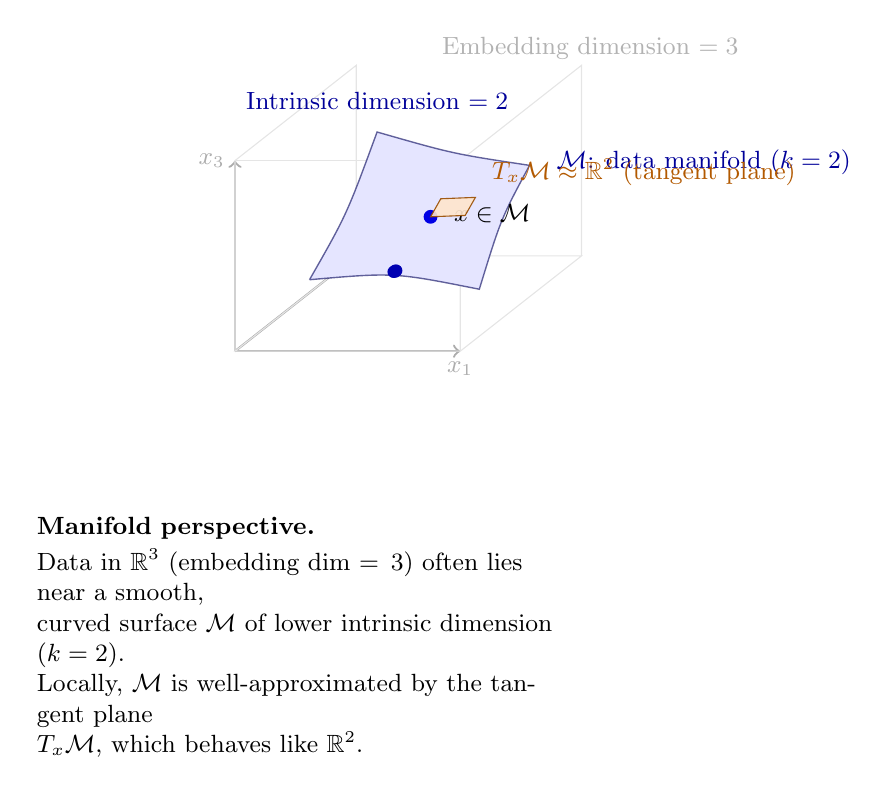
\begin{tikzpicture}[scale=2.2, every node/.style={font=\small}]

% --------- Axes setup (oblique 3D look) ----------
\coordinate (O)  at (0,0);
\coordinate (E1) at (1.30,0.00);  % x1 axis direction (absolute point)
\coordinate (E2) at (0.70,0.55);  % x2 axis direction
\coordinate (E3) at (0.00,1.10);  % x3 axis direction

% Axes
\draw[->,gray!65,thick] (O)--(E1) node[below] {$x_1$};
\draw[->,gray!65,thick] (O)--(E2) node[right] {$x_2$};
\draw[->,gray!65,thick] (O)--(E3) node[left]  {$x_3$};

% --------- Faint ambient box (embedding space hint) ----------
\coordinate (A)   at (O);
\coordinate (B)   at (E1);
\coordinate (C)   at (E2);
\coordinate (D)   at (E3);
\coordinate (BC)  at ($(E1)+(E2)$);
\coordinate (BD)  at ($(E1)+(E3)$);
\coordinate (CD)  at ($(E2)+(E3)$);
\coordinate (BCD) at ($(E1)+(E2)+(E3)$);

\draw[gray!20] (A)--(B)--(BC)--(C)--cycle;      % base parallelogram
\draw[gray!20] (A)--(D)--(CD)--(C);
\draw[gray!20] (B)--(BD)--(BCD)--(BC);
\draw[gray!20] (D)--(BD);

\node[gray!60,align=right] at ($(BCD)+(0.05,0.10)$) {Embedding dimension $=3$};

% --------- Curved 2D manifold (a bent sheet) ----------
\coordinate (m1) at ($(O)+0.25*(E1)+0.15*(E2)+0.30*(E3)$);
\coordinate (m2) at ($(O)+0.95*(E1)+0.25*(E2)+0.20*(E3)$);
\coordinate (m3) at ($(O)+0.85*(E1)+0.85*(E2)+0.55*(E3)$);
\coordinate (m4) at ($(O)+0.20*(E1)+0.80*(E2)+0.75*(E3)$);

% Control points for gentle curvature
\coordinate (c12a) at ($(m1)!0.50!(m2)+(0.00,0.07)$);
\coordinate (c23a) at ($(m2)!0.50!(m3)+(-0.02,0.05)$);
\coordinate (c34a) at ($(m3)!0.50!(m4)+(0.00,-0.03)$);
\coordinate (c41a) at ($(m4)!0.50!(m1)+(0.02,-0.05)$);

% Filled manifold surface
\fill[blue!10]
  (m1) .. controls ($(m1)!0.5!(m2)!1!(c12a)$) .. (m2)
       .. controls ($(m2)!0.5!(m3)!1!(c23a)$) .. (m3)
       .. controls ($(m3)!0.5!(m4)!1!(c34a)$) .. (m4)
       .. controls ($(m4)!0.5!(m1)!1!(c41a)$) .. (m1);

% Edge stroke for the manifold (subtle)
\draw[blue!35!black,opacity=0.6,line width=0.5pt]
  (m1) .. controls ($(m1)!0.5!(m2)!1!(c12a)$) .. (m2)
       .. controls ($(m2)!0.5!(m3)!1!(c23a)$) .. (m3)
       .. controls ($(m3)!0.5!(m4)!1!(c34a)$) .. (m4)
       .. controls ($(m4)!0.5!(m1)!1!(c41a)$) .. (m1);

\node[blue!60!black,anchor=west] at ($(m3)+(0.10,0.02)$) {$\mathcal{M}$: data manifold ($k=2$)};
\node[blue!60!black] at ($(m4)+(0.0,0.18)$) {Intrinsic dimension $=2$};

% --------- Sample data points lying on the manifold ----------
\foreach \t/\s in {0.15/0.20, 0.40/0.55, 0.65/0.35, 0.80/0.80, 0.55/0.75}{
  \coordinate (Aline) at ($ (m1)!\t!(m2) $);
  \coordinate (Bline) at ($ (m4)!\t!(m3) $);
  \coordinate (Ptemp) at ($ (Aline)!\s!(Bline) $);
  \coordinate (P)     at ($(Ptemp)!0.98!(c12a)$);
  \fill[blue!70!black] (P) circle (0.035);
}

% --------- A specific point x on the manifold ----------
\coordinate (x) at ($(m1)!0.55!(m3)$);
\fill[blue!90!black] (x) circle (0.04);
\node[anchor=west] at ($(x)+(0.08,0.02)$) {$x \in \mathcal{M}$};

% --------- Tangent plane at x (local linear approximation) ----------
% Two approximate tangent directions near x
\coordinate (t1) at ($(x)+0.23*(E1)-0.02*(E2)+0.02*(E3)$);
\coordinate (t2) at ($(x)-0.07*(E1)+0.25*(E2)+0.01*(E3)$);

% Small parallelogram around x using only calc-safe operations
\coordinate (tpA) at ($(x)$);
\coordinate (tpB) at ($ (x)!0.70!(t1) $);
\coordinate (tpD) at ($ (x)!0.70!(t2) $);
\coordinate (tpC) at ($ (tpB) + (tpD) - (x) $);

\fill[orange!20,draw=orange!60!black,opacity=0.9]
  (tpA)--(tpB)--(tpC)--(tpD)--cycle;

\node[orange!70!black,anchor=south west] at ($(tpC)+(0.04,0.01)$)
  {$T_x\mathcal{M} \approx \mathbb{R}^2$ (tangent plane)};

% --------- Legend / captions ----------
\node[align=left, text width=6.6cm, anchor=north west] at ($(O)+(-1.2,-0.9)$) {%
\textbf{Manifold perspective.}\\[2pt]
Data in $\mathbb{R}^3$ (embedding dim $=3$) often lies near a smooth,\\
curved surface $\mathcal{M}$ of lower intrinsic dimension ($k=2$).\\
Locally, $\mathcal{M}$ is well-approximated by the tangent plane\\
$T_x\mathcal{M}$, which behaves like $\mathbb{R}^2$.
};

\end{tikzpicture}
\end{document}
